\documentclass{beamer}
\usetheme{metropolis}
\usepackage{appendixnumberbeamer}
\usepackage{tabu}
\usepackage{listings}
\usepackage{hyperref}
%\usepackage{pgfplotsthemetol}
\hypersetup{colorlinks=true}

\newcommand{\jumbotron}[1]{ \centering \LARGE{#1} }
\newcommand{\citebook}{\tiny{Source: \emph{Introduction to Reproducible Science in R} -- Brian Lee Yung Rowe}}

\definecolor{graydark}{rgb}{0.3,0.3,0.3}
\definecolor{graymedium}{rgb}{0.5,0.5,0.5}
\definecolor{graylight}{rgb}{0.7,0.7,0.7}

\lstloadlanguages{bash}
\lstdefinestyle{custombash}{
  language=bash,
  frame=bt,
  otherkeywords={$},
  numberstyle=\tiny\color{graymedium},
  basicstyle=\footnotesize\ttfamily,
  stringstyle=\color{graydark},
  commentstyle=\color{graymedium},
  keywordstyle=\textbf\ttfamily,
  showstringspaces=false,
  numbers=left,
  breaklines=true
}
\lstset{style=custombash}


\title{How to Create a Development Environment for Reproducible Research} 
\date{\today} 
\author{Brian Lee Yung Rowe} 
\institute{Founder \& CEO, Pez.AI\\ CEO, FundKo} 

\begin{document} 
\maketitle 

\begin{frame}{Outline}
\begin{itemize}
\item Preliminaries
\item Demo!
\item Architecture
\item Process Automation

\end{itemize}
\end{frame}

\section{Preliminaries}

\begin{frame}{About Me}
\begin{itemize}
\item Founder \& CEO of \href{https://pez.ai}{Pez.AI}, productivity chatbots that make communication and coordination more efficient
\item CEO of \href{https://fundko.com}{FundKo}, P2P lender in Philippines using behavioral economics to improve lending outcomes
\item Author of \emph{Introduction to Reproducible Science in R}, to be published by Chapman and Hall/CRC Press
\item 6 years adjunct: NLP, machine learning, predictive analytics, mathematics
\item 14 years quantitative finance/investment management
\end{itemize}
\end{frame}



\begin{frame}[fragile]{Confirm Your Setup}
Confirm docker
\begin{lstlisting}
$ sudo docker --version
Docker version 19.03.8, build afacb8b7f0
\end{lstlisting}

Confirm \href{https://github.com/zatonovo/crant}{crant}
\begin{lstlisting}
$ which crant
/home/brian/workspace/crant/crant
\end{lstlisting}
\end{frame}


\begin{frame}{Poll: Environment + Skills}
Experience with Linux?
Experience with R?
Programming experience?

Take \href{}{poll} on your background

See \href{}{results in real-time}
\end{frame}



\section{Motivation}

\begin{frame}{Goal}
\alert{Spend less time setting up infrastructure and more time modeling}

The computing environment is repeatable. Do it right once, and reuse.
\end{frame}

\begin{frame}{Components}
\begin{itemize}
\item Docker - container technology
\item Linux - operating system
\item bash - command line shell
\item crant - project creation and build tool for R
\item make - build tool
\item git - version control
\item OpenCPU - REST API wrapper
\item Jupyter - notebook runtime
\item RMarkdown - Simple reports
\item Shiny - interactive reports
\end{itemize}
\end{frame}


\begin{frame}{Why Docker/Containers?}
Containers are lightweight, isolated computing environments that
\begin{itemize}
\item guarantee exact replicas
\item are easy to share
\item are easy to automate
\item are easy to orchestrate
\end{itemize}
\end{frame}


\begin{frame}{Why Linux?}
UNIX is the gift that keeps on giving
\begin{itemize}
\item 50 years old and still kicking it
\item \href{}{UNIX principles} are ubiquitous and timeless
\item Open source (accessible)
\item Many R commands borrow from UNIX commands (e.g, \lstinline|ls|, \lstinline|grep|)
\item Many Docker commands borrow from UNIX, make concepts (e.g., \lstinline|docker ps|)
\item Many git commands leverage UNIX concepts
\item Designed for headless operation
\end{itemize}
\end{frame}


\begin{frame}{Why Bash/Command Line?}
For repeatability and reproducibility, skip the GUI and go to the command line
\begin{itemize}
\item Every operation can be saved in a script and run in the future
\item Automatic documentation
\item Auditable
\item Version control
\item Minimize repetitive stress injuries!
\end{itemize}
\end{frame}


\begin{frame}{Why crant?}
Spend more time on analysis and less time on infrastructure

\begin{itemize}
\item Embraces data science workflow (ad hoc to structured development)
\item Batteries included (opencpu, jupyter, shiny)
\item Immediately runnable
\item Easily customized
\item Non-destructive
\item Mature - since 2012
\end{itemize}
\end{frame}



\section{Demo}
\begin{frame}[fragile]{Create New Project}
Make a directory

\begin{lstlisting}
$ mkdir -p caffeine/R
$ cd caffeine
\end{lstlisting}
\end{frame}

\begin{frame}{Do Data Science Stuff}
%\includegraphics[width=\linewidth]{images/}
\begin{itemize}
\item Explore dataset
\item Parse/normalize data
\item Make a model
\item etc
\end{itemize}
\end{frame}


\begin{frame}[fragile]{Initialize Package}
Use crant to initialize the package
\begin{lstlisting}
$ init_package -a 'Brian Lee Yung Rowe <r@zatonovo.com>' -t 'Caffeine Analysis of Coffee' -d 'This package predicts caffeine content of coffee'
\end{lstlisting}

Add dependencies to the Dockerfile
\begin{lstlisting}
$ sed -i '/FROM/a RUN rpackage htmltab' Dockerfile
\end{lstlisting}

\end{frame}


\begin{frame}[fragile]{Initialize Repository}
Initialize an empty repository for your project
\begin{lstlisting}
$ git init
\end{lstlisting}

See what crant created for you
\begin{lstlisting}
$ git status
\end{lstlisting}

Add and commit files to your repo
\begin{lstlisting}
$ git add .
$ git commit -am "Initial commit"
\end{lstlisting}
\end{frame}


\begin{frame}[fragile]{Build and Run REST Server}

Verify package builds locally (optional)
\begin{lstlisting}
$ crant -x
\end{lstlisting}

Build image (and build package inside image)
\begin{lstlisting}
$ sudo make run
\end{lstlisting}

A new container is created from the image.
Visit web page \href{http://127.0.0.1:8004/ocpu/}{http://127.0.0.1:8004/ocpu/}

\begin{lstlisting}
$ curl -H "Content-Type: application/json" \
  http://127.0.0.1:8004/ocpu/library/coffee/R/trim/json \
  -d '{"x":" adfljk "}'
["adfljk"]
\end{lstlisting}
\end{frame}


\begin{frame}[fragile]{Attach bash Session}
Inspect a running container via bash

\begin{lstlisting}
$ sudo make bash
\end{lstlisting}
\end{frame}


\begin{frame}[fragile]{Run Notebook Server}
Stop web server
\begin{lstlisting}
$ sudo make stop
\end{lstlisting}

Start notebook server
\begin{lstlisting}
$ sudo make notebook

Copy/paste this URL into your browser when you connect for the first time,
    to login with a token:
        http://localhost:8888/?token=ccdaaf6e9222ccfc9640200661755377f0c83cd927f875a6
\end{lstlisting}
\end{frame}


\begin{frame}[fragile]{Exercise: Try It}
Try on your own project

\alert{Use web conference chat to ask questions}
\end{frame}



\section{Infrastructure}

\begin{frame}{Virtualization and Containers}
History is a spiral

\begin{columns}[T]
\begin{column}{.33\linewidth}
1970s

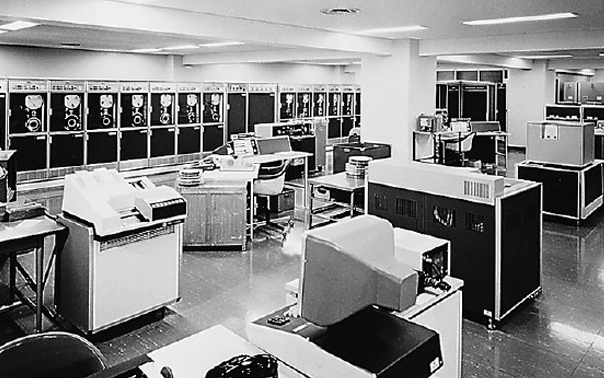
\includegraphics[width=\linewidth]{images/mainframe_1975}

Dumb terminals - mainframes
\end{column}

\begin{column}{.3\linewidth}
late 1970s - 2000s

%https://www.smithsonianmag.com/smithsonian-institution/august-3-1977-the-trs-80-personal-computer-goes-on-sale-186379/
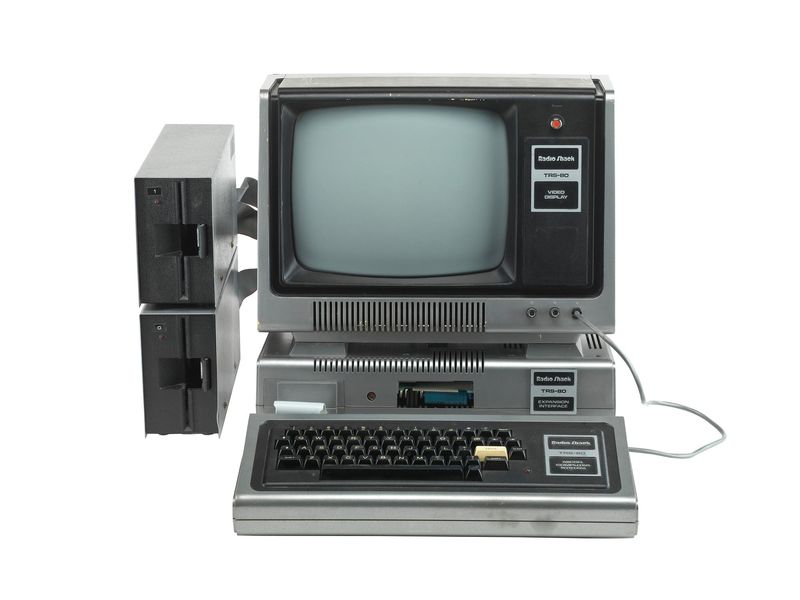
\includegraphics[trim=0 9mm 0 9mm,clip, width=\linewidth]{images/trs-80}

Personal computers
\end{column}

\begin{column}{.33\linewidth}
2000s - present
%https://engineering.fb.com/production-engineering/introducing-data-center-fabric-the-next-generation-facebook-data-center-network/
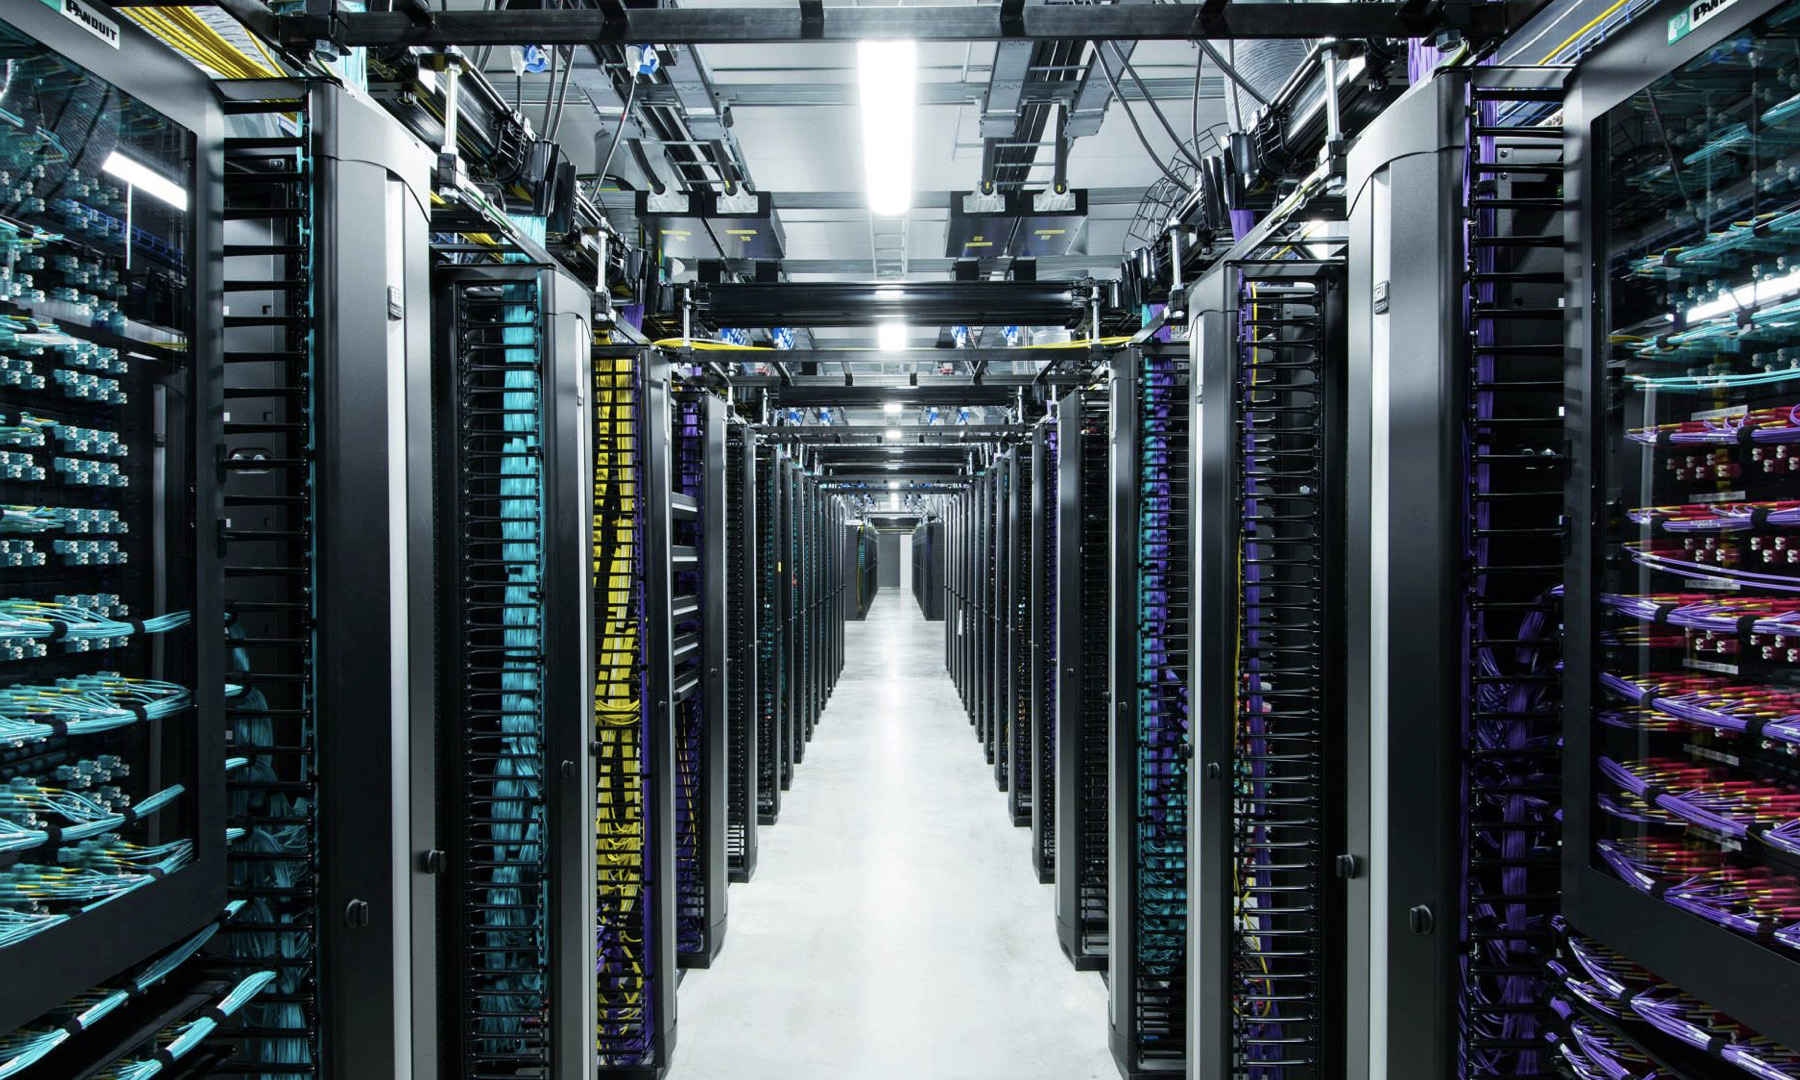
\includegraphics[width=\linewidth]{images/datacenter_fb}

Smart terminals - mainframes
\end{column}
\end{columns}
\end{frame}

\begin{frame}{Docker}
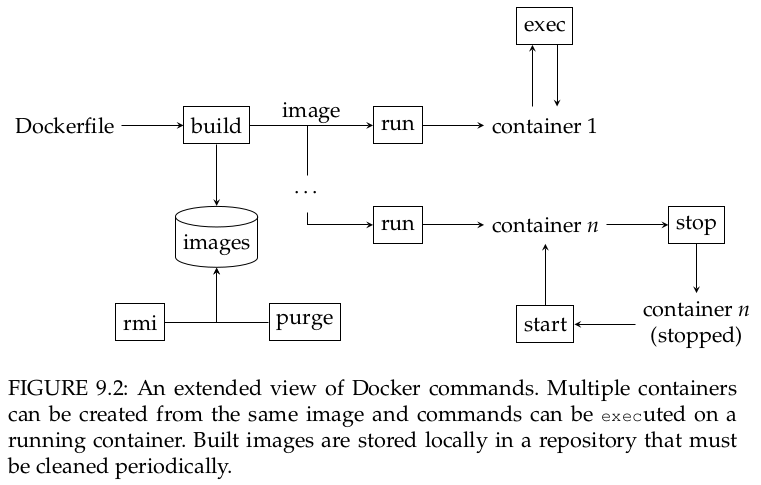
\includegraphics[width=\linewidth]{images/docker_commands}
\end{frame}

\begin{frame}{Docker Mnemonic: OOP}
Images are to containers as classes are to objects

\alert{A container is an instance of an image}
\end{frame}

\begin{frame}{Docker Commands}

\begin{tabu} to \linewidth{lX}
Command & Description\\
\hline
\lstinline|docker run| & Start a new container\\
\lstinline|docker stop| & Stop a running container\\
\lstinline|docker exec| & Attach a process to a running container\\
\lstinline|docker ps| & View running containers\\
\lstinline|docker images| & View images on workstation\\
\lstinline|docker push| & Push an image to a repository (e.g., Docker Hub)\\
\lstinline|docker pull| & Pull an image from a repository\\
\end{tabu}
\end{frame}




\begin{frame}[fragile]{Version Control}
Source code management facilitates:

\begin{itemize}
\item change management
\item collaboration
\item auditing
\item recovery
\end{itemize}
\end{frame}


\begin{frame}[fragile]{Distributed Version Control}
git is a decentralized SCM with \alert{free branches}

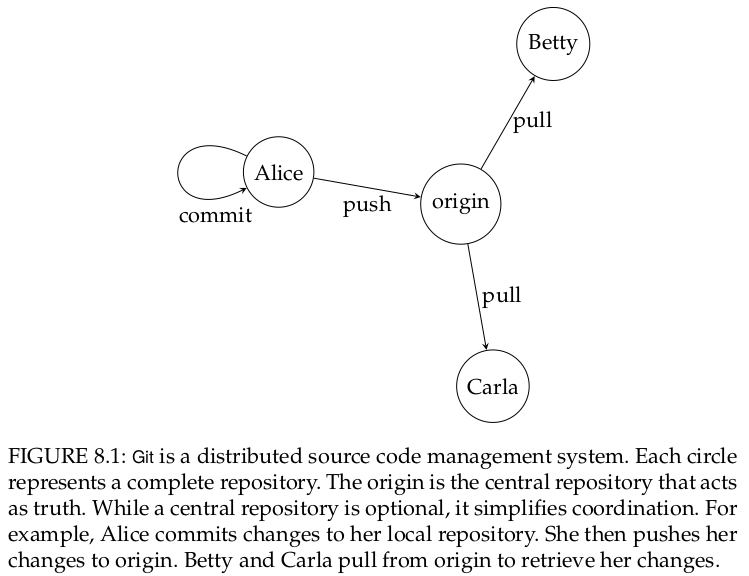
\includegraphics[width=.8\linewidth]{images/git_interactions}
\end{frame}

\begin{frame}[fragile]{Git Concepts}

\begin{itemize}
\item commits
\item branches (master, other)
\item remotes (origin, other)
\end{itemize}

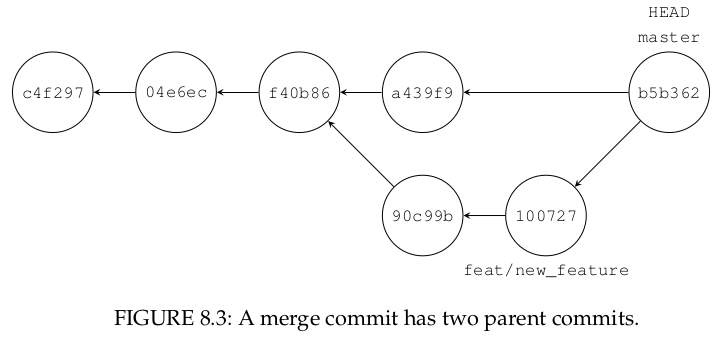
\includegraphics[width=.8\linewidth]{images/git_branches}
\end{frame}

\begin{frame}[fragile]{Git Commands}
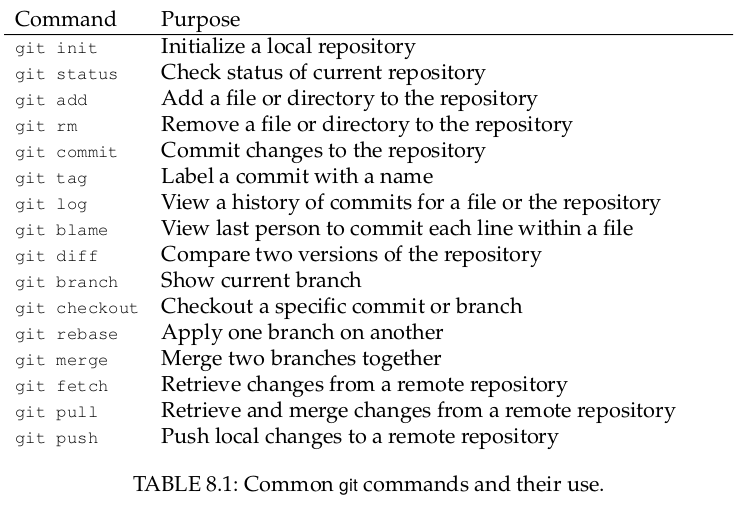
\includegraphics[width=\linewidth]{images/git_commands}
\end{frame}



\begin{frame}[fragile]{Exercise: Try It}

\begin{enumerate}
\item Make some changes
\item Use \lstinline|git status| to view current state of repo
\item Commit changes with \lstinline|git commit|
\end{enumerate}

\alert{Use web conference chat to ask questions}
\end{frame}


\section{Architecture}

\begin{frame}{System Architecture}
Crant configures a basic, reusable system from common tools

\tiny
\begin{tikzpicture}
\node (arch) at (0,0) {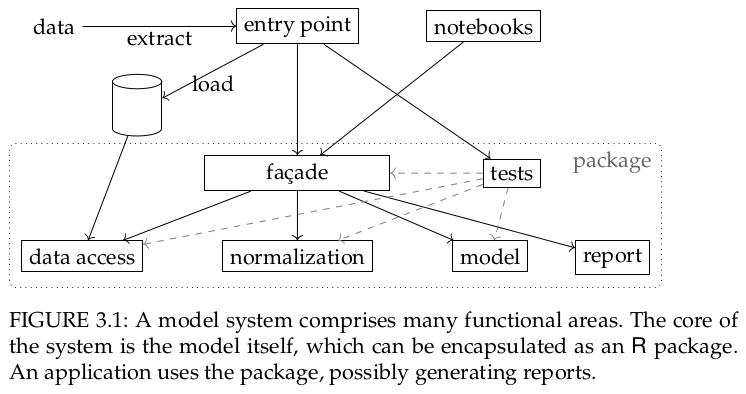
\includegraphics[width=\linewidth]{images/model_system}};

\pause
\node[draw,rectangle, minimum width=3cm] at (-1.1,1) {REST API (OpenCPU)};
\node[draw,rectangle, minimum width=1.2cm] at (3.45,-0.4) {Shiny};

\end{tikzpicture}

%Makefile manages high-level operations
\end{frame}


\begin{frame}{Pipeline Architecture}
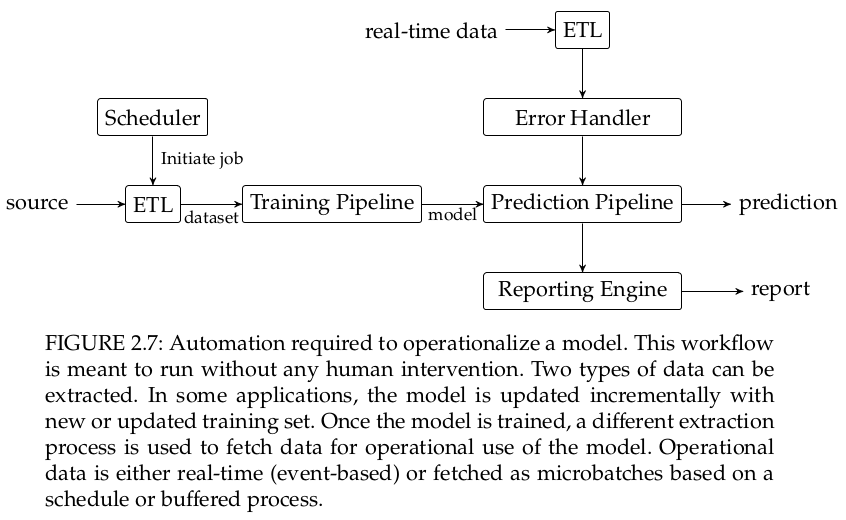
\includegraphics[width=\linewidth]{images/o16n_pipeline}
\end{frame}

\begin{frame}{Project Structure}
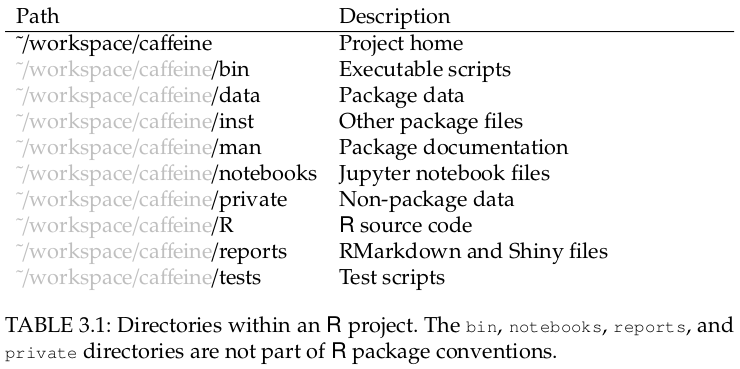
\includegraphics[width=\linewidth]{images/directory_structure}
\end{frame}


\begin{frame}{The onion and the graph}
R is a functional programming language.
Avoid excessive use of object-oriented programming techniques.

\begin{itemize}
\item Use a graph to organize your system
\item Create layers and keep layers consistent
\item Use fa\c{c}ades to simplify entry points
\item Remember, mathematics is a functional programming language
\end{itemize}

\end{frame}



\section{Software Development Workflows and Tools}

\begin{frame}{crant}
Raison d'\^{e}tre: command line control of R projects for automation

\begin{itemize}
\item Build tool (build, test, manage versions)
\item Package "manager"
\item Project initialization (Docker, make, R package, Travis CI)
\item Shiny initialization
\end{itemize}
\end{frame}


\begin{frame}{Crant Is For Model Development}
Crant is designed with model development in mind

Unlike software development, model development
\begin{itemize}
\item often has no master plan (driven by the analysis)
\item may result in a dead-end
\item structure is added later in process
\end{itemize}
\end{frame}


\begin{frame}{Controller}
Makefile acts as controller of the system
\begin{itemize}
\item \lstinline|make all| - build image and package
\item \lstinline|make run| - start container and run web server
\item \lstinline|make stop| - stop container
\item \lstinline|make notebook| - start notebook server
\item \lstinline|make shiny| - start shiny server
\item \lstinline|make bash| - start bash session within running container
\item \lstinline|make r| - start container and run R session
\end{itemize}
\end{frame}


\begin{frame}{Testing}
Testing helps you:


\begin{itemize}
\item provide evidence that code works as expected
\item increase likelihood of reproducible code
\item limit damage when refactoring code
\item document how to use functions
\end{itemize}
\end{frame}


\begin{frame}{Testing Lesson}
\centering
\huge
\alert{Focus testing effort on functions with high variability in input}
\end{frame}


\begin{frame}[fragile]{Testit}
\begin{lstlisting}
assert("trim removes whitespace at beginning and end of string", {
  x <- c(" padding ", "hello.", " \n weird stuff ")
  exp <- c("padding", "hello.", "weird stuff")
  act <- trim(x)

  (all(act == exp))
})
\end{lstlisting}
\end{frame}


\begin{frame}[fragile]{Running Tests}
\lstinline|init_package| creates test stubs and example 
in \lstinline|tests/testit|

\begin{lstlisting}
$ make all
\end{lstlisting}
\end{frame}



\begin{frame}[fragile]{Logging}
Log messages help you:

\begin{itemize}
\item peer into the state of your program
\item observe the progress of a process
\item estimate the run time of a process
\item troubleshoot a buggy process
\end{itemize}
\end{frame}


\begin{frame}{Logging Lesson}
\centering
\huge
\alert{Use log messages before the debugger}
\end{frame}

\begin{frame}[fragile]{Logging Framework}
\lstinline|init_package| includes 
\href{https://github.com/zatonovo/futile.logger}{\lstinline|futile.logger|}
for logging.

\begin{itemize}
\item Based on log4j (as is Python logging)
\item Simplified semantics for non-developers :)
\item Default configuration is usable!
\end{itemize}

\begin{lstlisting}
> flog.info("Hello")
\end{lstlisting}
\end{frame}


\begin{frame}[fragile]{Logging Concepts}

\begin{lstlisting}
> flog.threshold(WARN)
> flog.info("This won't display")
\end{lstlisting}

\begin{itemize}
\item loggers - object that holds a configuration
\item thresholds - defines which log levels to display
\item log levels - severity of log message
\item appenders - where to write log messages
\item formatters - how to format log messages
\end{itemize}

\end{frame}



\begin{frame}[fragile]{Debugging}
Manual control of a process

\begin{itemize}
\item Inspect state of system
\item Observe execution path in real-time
\item Try alternative logic
\item Not repeatable
\end{itemize}
\end{frame}


\begin{frame}{Debugging Lesson}
\centering
\huge
\alert{Use the debugger as a last resort}
\end{frame}


\begin{frame}[fragile]{Debugging Concepts}
\begin{itemize}
\item Mark a function for debugging: \lstinline|debug()|
\item Start debugger at specific line of code: \lstinline|browser()|
\end{itemize}

\end{frame}



\begin{frame}[fragile]{Profiling}
Measure compute time of slow code

\begin{itemize}
\item logging
\item home grown
\item formal profiler
\end{itemize}
\end{frame}



\section{Modeling Workflows}

\begin{frame}{Training Pipeline}

\begin{itemize}
\item Use bash scripts as glue
\item Define options with \lstinline|getopts|
\end{itemize}
\end{frame}


\begin{frame}{Prediction API}

\begin{itemize}
\item Use cases
\item Scheduling, lambdas
\item Interactive charts
\end{itemize}
\end{frame}



\begin{frame}[fragile]{Interactive Notebooks}

\begin{itemize}
\item Interactive $\neq$ automated
\item Only appropriate for data scientist audience
\item Minimize code development in notebooks
\end{itemize}

\begin{lstlisting}
$ sudo make notebook
\end{lstlisting}
\end{frame}


\begin{frame}[fragile]{Interactive Analysis: Shiny}
\begin{lstlisting}
$ cd $project
$ init_shiny
$ sudo make shiny
\end{lstlisting}
\end{frame}


\begin{frame}[fragile]{Report Generation: Rmarkdown}
Create document in \lstinline|reports|
\begin{lstlisting}
---
title: A simple report
output: pdf_document
---
# Abstract
The abstract

# Methodology
```{r}
rnorm(4)
```
\end{lstlisting}

Create report
\begin{lstlisting}
> rmarkdown::render('reports/myreport.Rmd')
\end{lstlisting}
\end{frame}



\begin{frame}{Thank You}
Slides: \href{https://github.com/muxspace/sdss_2020}{Github}\\
Website: \href{https://cartesianfaith.com}{cartesianfaith.com}\\
Twitter: @cartesianfaith\\
Questions: \href{mailto:rowe@zatonovo.com}{rowe@zatonovo.com}

Let me know if you are interested in my

\begin{itemize}
\item Twitch channel for real-time data science help/review
\item book \emph{Introduction to Reproducible Science in R}
\item productivity chatbots
\item alternative lending models
\end{itemize}
\end{frame}

%\appendix
%
%\begin{frame}[fragile]{Debugging Docker Images}
%If an image won't successfully build, you can inspect an intermediate layer
%
%\begin{lstlisting}
%$ sudo docker run -it --rm 0a871620efa2 bash
%\end{lstlisting}
%\end{frame}

\end{document}
